\section{Multi-Objective Optimization}
In the optimization of structural systems, it may sometimes be necessary to simultaneously optimize multiple conflicting objectives. This section will examine multi-objective optimization methods and applications. \sidenote{In multi-objective optimization, instead of a single optimal solution, a set of Pareto-optimal solutions is obtained.
To better understand multi-objective optimization, the example code in the link can be examined.

\qrcode[height=1in]{https://github.com/btayfur/structural-optimization/blob/main/Code/Examples/Exmp5/}}

\subsection{Foundations of Multi-Objective Optimization}
Simultaneous optimization of multiple objective functions:

\begin{tcolorbox}[title=Basic Concepts]
\begin{itemize}
    \item \textbf{Pareto Optimality:} Dominant solutions
    \item \textbf{Trade-off:} Compromise between objectives
    \item \textbf{Decision Making:} Solution selection
    \item \textbf{Weighting:} Prioritization of objectives
\end{itemize}
\end{tcolorbox}

\subsection{Mathematical Formulation}
General structure of multi-objective optimization problem:

\begin{equation}
\begin{aligned}
& \text{minimize} & & \mathbf{F}(\mathbf{x}) = [f_1(\mathbf{x}), f_2(\mathbf{x}), \ldots, f_k(\mathbf{x})]^T \\
& \text{subject to} & & g_i(\mathbf{x}) \leq 0, & & i = 1,\ldots,m \\
& & & h_j(\mathbf{x}) = 0, & & j = 1,\ldots,p \\
& & & \mathbf{x}^L \leq \mathbf{x} \leq \mathbf{x}^U
\end{aligned}
\end{equation}

\begin{marginfigure}
\centering
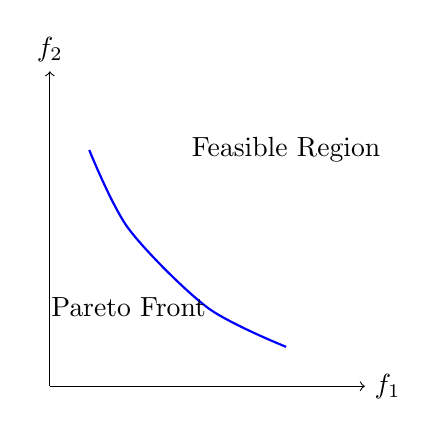
\begin{tikzpicture}
\draw[->] (0,0) -- (4,0) node[right] {$f_1$};
\draw[->] (0,0) -- (0,4) node[above] {$f_2$};
\draw[blue,thick] plot[smooth] coordinates {(0.5,3) (1,2) (2,1) (3,0.5)};
\node at (3,3) {Feasible Region};
\node at (1,1) {Pareto Front};
\end{tikzpicture}
\caption{Example of Pareto front}
\end{marginfigure}

\subsection{Solution Approaches}
The examination of basic strategies used in solving multi-objective optimization problems offers different approaches depending on how the problem is handled. That is, essentially, the decision-maker here is the engineer themselves. Whether the objective functions are superior to each other or their proportionality affects this decision and the strategy to be chosen.

\subsubsection{Scalarization Methods}
These are approaches that transform the multi-objective optimization problem into a single-objective problem. These methods combine multiple objectives to make the problem more easily solvable. Scalarization methods are widely used in engineering problems due to their quick and easy implementation. However, determining appropriate weights can complicate the process as it directly affects the quality of the solution.

\begin{tcolorbox}[title=Common Scalarization Methods]
\begin{itemize}
    \item \textbf{Weighted Sum Method:} $F(x) = \sum_{i=1}^{k} w_i f_i(x)$
    \item \textbf{$\varepsilon$-Constraint Method:} One objective is optimized while others are defined as constraints
    \item \textbf{Goal Programming:} $\min \sum_{i=1}^{k} w_i |f_i(x) - T_i|$ (where $T_i$ are target values)
\end{itemize}
\end{tcolorbox}

\subsubsection{Pareto-Based Approaches}
Pareto-based approaches aim to find all Pareto-optimal solutions or a good representation of them. These methods allow exploring a larger portion of the solution space and offer more alternatives to the decision-maker. Pareto-based approaches are particularly effective when evolutionary algorithms are used.

Basic components of Pareto-based approaches are:
\begin{itemize}
    \item \textbf{Dominance Relation:} Determining whether one solution is better than another
    \item \textbf{Diversity Mechanisms:} Techniques ensuring homogeneous distribution of solutions along the Pareto front
    \item \textbf{Elite Strategies:} Mechanisms ensuring preservation of good solutions
\end{itemize}

\begin{marginfigure}
\centering
\begin{tikzpicture}
\draw[->] (0,0) -- (4,0) node[right] {$f_1$};
\draw[->] (0,0) -- (0,4) node[above] {$f_2$};
\draw[blue,thick] plot[smooth] coordinates {(0.5,3) (1,2) (2,1) (3,0.5)};
\filldraw[red] (0.5,3) circle (2pt);
\filldraw[red] (1,2) circle (2pt);
\filldraw[red] (2,1) circle (2pt);
\filldraw[red] (3,0.5) circle (2pt);
\filldraw[gray] (1.5,2.5) circle (2pt);
\filldraw[gray] (2.5,1.5) circle (2pt);
\draw[->] (1.5,2.5) -- (1.1,2.1);
\node at (1.2,2.8) {Dominated};
\end{tikzpicture}
\caption{Pareto dominance concept}
\end{marginfigure}

\subsubsection{Interactive Methods}
Interactive methods involve the decision-maker in the optimization process, narrowing the solution space according to their preferences. This approach integrates the decision-maker's knowledge and experience into the algorithm's operation. Interactive methods are valuable in complex engineering problems, particularly in terms of incorporating expert knowledge into the solution process.

Advantages of interactive approaches:
\begin{itemize}
    \item Ability to directly reflect decision-maker's preferences into the process
    \item Directing computational resources to the solution region of interest
    \item Obtaining more meaningful and applicable results
\end{itemize}

\subsection{Evolutionary Multi-Objective Optimization Algorithms}
The application of evolutionary algorithms to multi-objective optimization problems provides significant advantages over classical methods. These algorithms stand out with their ability to produce multiple solutions at once, handle complex objective functions, and effectively search large solution spaces.

\subsubsection{NSGA-II (Non-dominated Sorting Genetic Algorithm)}
NSGA-II is one of the most widely used algorithms in the field of multi-objective evolutionary optimization. With its dominance sorting and crowding distance calculation mechanisms, it provides both convergence to Pareto-optimal solutions and diversity among solutions. NSGA-II operates quite efficiently with $O(MN^2)$ computational complexity and has been successfully applied in many engineering problems.

Basic components of NSGA-II:
\begin{itemize}
    \item \textbf{Fast Non-dominated Sorting:} Sorts solutions in the population according to dominance relation
    \item \textbf{Crowding Distance:} Maintains diversity among solutions at the same dominance level
    \item \textbf{Binary Tournament Selection:} Selection mechanism based on dominance level and crowding distance
\end{itemize}

\subsubsection{MOEA/D (Multiobjective Evolutionary Algorithm based on Decomposition)}
MOEA/D is an evolutionary algorithm that solves the multi-objective optimization problem by decomposing it into a series of single-objective subproblems. Each subproblem is optimized simultaneously by sharing information with neighboring subproblems. This approach is particularly effective in problems with many objective functions and is computationally efficient.

Advantages of MOEA/D:
\begin{itemize}
    \item Effective information sharing through neighborhood structure
    \item Suitability for problems with many objective functions
    \item Ability to use different decomposition methods (Tchebycheff, weighted sum, etc.)
\end{itemize}

\subsubsection{SPEA2 (Strength Pareto Evolutionary Algorithm)}
SPEA2 is an evolutionary algorithm that stores and refines Pareto-optimal solutions using a fixed-size archive. The algorithm considers both dominance relation and solution density by assigning a fitness value to each solution. SPEA2 is preferred particularly because it establishes a good balance between diversity and convergence.

Important features of SPEA2:
\begin{itemize}
    \item \textbf{Strength Value:} Measures how many solutions a solution dominates
    \item \textbf{Density Estimation:} Calculated using K-nearest neighbor method
    \item \textbf{External Archive:} Efficiently stores and updates Pareto-optimal solutions
\end{itemize}

\subsection{Decision Making Processes}
Multi-objective optimization produces a set of Pareto-optimal solutions, and a choice must be made among these solutions. The decision-making process is a critical part of the optimization process and can be supported by various approaches.

\subsubsection{Solution Selection Criteria}
Various criteria can be used when selecting among Pareto-optimal solutions:
\begin{itemize}
    \item \textbf{Distance Measures:} Solution closest to ideal point (e.g., Euclidean distance, Tchebycheff distance)
    \item \textbf{Satisfaction Level:} Solutions satisfying threshold values determined for each objective
    \item \textbf{Relative Improvement:} Rate of improvement of one objective relative to another (trade-off analysis)
    \item \textbf{Risk Analysis:} Reliability of solutions under uncertainty
\end{itemize}

\begin{tcolorbox}[title=Example: Weighted Tchebycheff Metric]
\begin{equation}
d(F, F^*) = \max_{i=1,...,k} \{w_i \cdot |F_i - F_i^*|\}
\end{equation}
Where $F^*$ is the ideal point, $w_i$ are the weights of objectives, and $F_i$ is the $i$th objective value of the current solution.
\end{tcolorbox}

\subsubsection{Weighting Strategies}
Various weighting strategies can be used to determine the relative importance of objectives:
\begin{itemize}
    \item \textbf{Direct Assignment:} Direct weight assignment by decision-maker
    \item \textbf{AHP (Analytic Hierarchy Process):} Weight determination through pairwise comparisons
    \item \textbf{Entropy-Based Methods:} Weight calculation based on data distribution
    \item \textbf{TOPSIS:} Weighting by similarity to ideal solution
\end{itemize}

\subsubsection{Comparison Between Solutions}
Comparing different Pareto-optimal solutions helps the decision-maker choose the solution suitable for their preference:
\begin{itemize}
    \item \textbf{Visualization Techniques:} Parallel coordinate plots, star diagrams, heat maps
    \item \textbf{Sensitivity Analysis:} Effect of parameter changes on solution
    \item \textbf{Robust Evaluation:} Performance of solutions under uncertainty
    \item \textbf{Life Cycle Analysis:} Long-term performance and cost evaluation
\end{itemize}

\begin{marginfigure}
\centering
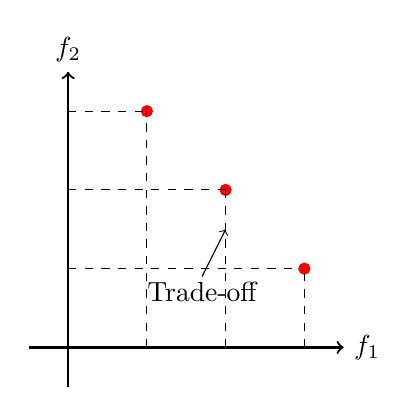
\begin{tikzpicture}
\draw[->,thick] (-0.5,0) -- (3.5,0) node[right] {$f_1$};
\draw[->,thick] (0,-0.5) -- (0,3.5) node[above] {$f_2$};
\filldraw[red] (1,3) circle (2pt);
\filldraw[red] (2,2) circle (2pt);
\filldraw[red] (3,1) circle (2pt);
\draw[dashed] (1,0) -- (1,3);
\draw[dashed] (0,3) -- (1,3);
\draw[dashed] (2,0) -- (2,2);
\draw[dashed] (0,2) -- (2,2);
\draw[dashed] (3,0) -- (3,1);
\draw[dashed] (0,1) -- (3,1);
\node at (1.7,0.7) {Trade-off};
\draw[->] (1.7,0.9) -- (2,1.5);
\end{tikzpicture}
\caption{Trade-off analysis between Pareto solutions}
\end{marginfigure}

\subsection{Performance Metrics in Multi-Objective Optimization}
\subsubsection{Hypervolume}
Hypervolume is one of the most common metrics used to evaluate the performance of multi-objective optimization algorithms. This metric expresses the measure of the area or volume covered by the Pareto front relative to a reference point. A higher hypervolume value indicates that the algorithm has found a better Pareto front, as this means a larger portion of the solution space is covered.

\subsubsection{IGD (Inverted Generational Distance)}
Inverted Generational Distance (IGD) is a measure of the distance between the true Pareto front and the solution set found by the algorithm. This metric shows how close the found solutions are to the true Pareto front and how well they represent the front. A lower IGD value indicates that the algorithm has found solutions closer to and better distributed along the true Pareto front.

\subsubsection{Spread (Diversity)}
The spread metric is a measure of the distance between points in the solution set and shows how homogeneously solutions are distributed along the Pareto front. This metric evaluates how well the algorithm explores the solution space and can offer various alternatives. Lower spread values are preferred for a uniformly distributed Pareto front.

\subsubsection{Computation Time}
Computation time measures the time spent by an algorithm to reach a solution. This metric is important for evaluating the efficiency of an algorithm and its usability in practical applications. Especially in complex engineering problems, algorithms that can provide good results in a reasonable time are preferred. Computation time can vary depending on the complexity of the algorithm, problem size, and application environment. \sidenote{Since this parameter is quite relative, it does not always provide reliable results. Today, more modern metrics such as CPU Time are used.} 